\section{センサノードグループ再構成のアプローチ}

% ---自律型再グループ化 ---
\subsection{自律型再グループ化}
研究課題4.3における,集約ノードの消費電力負担が増加する課題を解決するため,グループ内で,GLを交代し電力の平準化を図る自律型グループ化について述べる.全センサノードは,消費電力見積もりのため,LoRaWAN及びBLEでの通信回数を保持する.消費電力量は下記モデル式をもとに見積もり可能である.下記にシーケンス(図\ref{fig:group_reconstruction_independently}参照)を示す.

\begin{enumerate}
    \item 次のGLノードを選出するため,GMノードはセンサデータとともに,通信回数をデータに載せる(図\ref{fig:group_reconstruction_independently}シーケンス番号1-2参照).
    \item GLノードはGMノードの消費電力量を見積もり,バッテリー容量が最も高い(消費電力量の少ない)センサノードを次のGLとして選出する(図\ref{fig:group_reconstruction_independently}シーケンス番号3参照).
    \item GLノードはGMノードとの通信を切断する際に,GMノードへ次のGLノードのサービスUUIDを通知する(図\ref{fig:group_reconstruction_independently}シーケンス番号4-5参照).
    \item その後,データを集約しGWノードへ送信する(図\ref{fig:group_reconstruction_independently}シーケンス番号6参照).
\end{enumerate}

これにより,グループ内でのセンサノードの消費電力を平準化が見込める.

\begin{figure}[]
    \begin{center}
    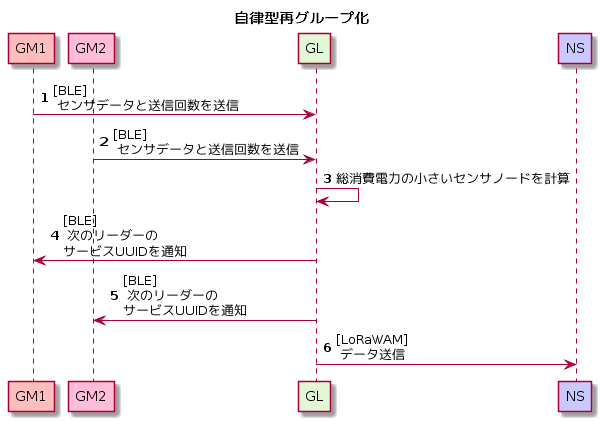
\includegraphics[width=14cm]{figures/v2.0/自律型再グループ化.png}
    \caption{自律型再グループ化}
    \label{fig:group_reconstruction_independently}
    \end{center}
\end{figure}

% --- 集中型再グループ化 ---
\subsection{集中型再グループ化}
提案手法では,WSN内にセンサノードが追加されていくと,初期に構築したグループでは最適でない場合が考えられる.そのため,グループの構成を変更し,WSN全体での電力の平準化を図る集中型グループ化について述べる.そのため,GWノードはセンサノードから取得したデータ(デバイス固有ID・信号強度)を用いて最適なグループを再構成する.下記にシーケンス(図\ref{fig:group_reconstruction_concentrately}参照)を示す.

\begin{enumerate}
    \item GMノードは,定常時と同様センサデータをGLノードへ送信する(図\ref{fig:group_reconstruction_concentrately}シーケンス番号1参照).
    \item GWノードは,データとして各センサノードの異種無線利用回数から消費電力量を算出しグループを再構成する(図\ref{fig:group_reconstruction_concentrately}シーケンス番号2-3参照).
    \item GWノードは,グループを再構成した際に再構成があれば通知する(図\ref{fig:group_reconstruction_concentrately}シーケンス番号4参照).
    \item GLノードは,GMノードに新しいリーダーのサービスUUIDを通知する.
\end{enumerate}

これにより,センサネットワーク全体の消費電力を平準化でき,センサ交換機会の削減が見込める.

\begin{figure}[]
    \begin{center}
    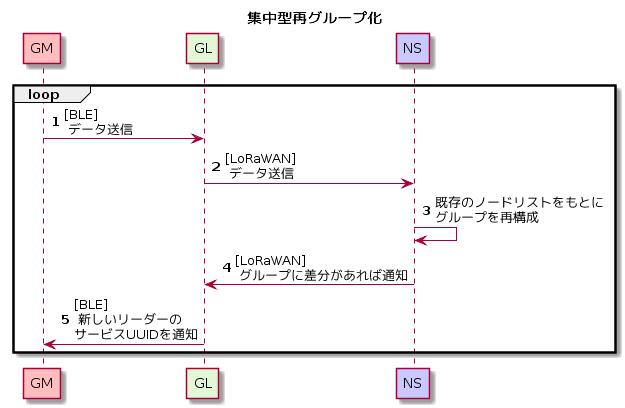
\includegraphics[width=14cm]{figures/v2.0/集中型再グループ化.png}
    \caption{集中型再グループ化}
    \label{fig:group_reconstruction_concentrately}
    \end{center}
\end{figure}